\chapter{Funciones de Bessel}

Cuando resolvemos la ecuación de Helmholtz en coordenadas cilíndricas, obtenemos una EDO para la coordenada radial, que bajo el cambio de variable $x = n\rho$, tomará la forma
% \begin{equation}
%     \rho \frac{d}{d\rho}\left( \rho \frac{dP}{d\rho} \right) + (n^2\rho^2 - m^2)P = 0 \ .
% \end{equation}
%
% Haciendo el cambio de variable $x = n\rho$, $\frac{d}{dx} = \frac{1}{n} \frac{d}{d\rho}$, con lo que la ecuación tomará la forma
\begin{equation}\label{eq:EDO_Bessel}
    x^2 \frac{d^2y}{dx^2} + x \frac{dy}{dx} + (x^2 - m^2) y = 0 \ ,
\end{equation}
conocida como la \textbf{ecuación de Bessel}.
% \begin{equation}
%     x^2 \frac{d^2y}{dx^2} + x \frac{dy}{dx} + (x^2 - m^2) y = 0 \ .
% \end{equation}

Si bien, al surgir del desarrollo de la ecuación de Helmholtz, se ha impuesto que $m$ es un valor entero, esta no es una restricción propia de la EDO de Bessel, por lo que comúnmente se denota a esta constante como $\nu$, la que puede tomar \emph{valores reales no negativos}\footnote{Comúnmente, se utilizan letras latinas para denotar números enteros, y letras griegas para números reales.}.

\section{Funciones de Bessel}

\subsection{Resolviendo la ecuación de Bessel mediante el método de Series}

En la EDO de Bessel, $P(x) = 1/x$ y $Q(x) = 1/x^2$, de modo que es claro que $x = 0$ es un punto \emph{singular regular}, pues $x P(x)$ y $x^2 Q(x)$ son analíticas en $x = 0$. Dado el tipo de singularidad, el teorema de Fuchs \ref{teo:Fuchs} nos asegura la existencia de una solución para la EDO mediante el método de Frobenius. Así, proponemos una solución de la forma
%
% Dado que $x=0$ es un punto \emph{singular irregular} de la ecuación de Bessel, podemos utilizar el método de Frobenius y proponer una solución de la forma
\begin{equation}\label{eq:solucion_serie_Bessel}
    y(x) = \sum_{k = 0}^\infty a_k x^{s+k} \ ,
\end{equation}
que tras derivarla, podemos incluirla en la ecuación de Bessel, obteniendo
\begin{equation}
    \sum_{k = 0}^\infty a_k (s + k)(s+ k - 1)x^{k + s} + \sum_{k = 0}^\infty a_k (s+k) x^{s+k} + \sum_{k = 0}^\infty a_{k} x^{s+k + 2} - \sum_{k = 0}^\infty a_k \nu^2 x^{s+k} = 0 \ .
\end{equation}

Haciendo $k = 0$, obtenemos el coeficiente que acompañará a $x^s$, la potencia de $x$ más pequeña que aparecerá al lado izquierdo de la ecuación, de modo que, como en general $x^s \neq 0$, tenemos
\begin{equation}
    a_0 \left[ s(s-1) + s - \nu^2 \right] = 0 \ ,
\end{equation}
y como por definición $a_0 \neq 0$, obtenemos la \textbf{ecuación indicial}
\begin{equation}
    s^2 - \nu^2 = 0 \ ,
\end{equation}
cuyas soluciones son $s = \pm \nu$.

Haciendo lo mismo para $k = 1$, tenemos la ecuación
\begin{equation}
    a_1\left[ (s+1)s + s + 1 - \nu^2 \right] = 0 \ ,
\end{equation}
que puede ser reescrito como
\begin{equation}
    a_1(s + 1 - \nu)(s + 1 + \nu) = 0 \ ,
\end{equation}
y como anteriormente impusimos que $s=\pm \nu$, tendremos que
\begin{equation}
    a_1 (1 + 2\nu) = 0 \ ,
\end{equation}
de modo al suponer que $\nu \neq -1/2$, requerimos que $a_1 = 0$.

Siguiendo el mismo proceso con los siguientes términos, podemos llegar a la relación de recurrencia
\begin{equation}
    a_{k + 2} = -a_k \frac{1}{(s+\nu+(k+2))(s-\nu+(k+2))} \ .
\end{equation} 
Es más, ya que los coeficientes impares se anulan al ser $a_1 = 0$, podemos escribir la relación de recurrencia únicamente para los coeficientes pares, de modo que
\begin{equation} \label{eq:recurrencia_Bessel}
    a_{2k} = (-1)^k \frac{1}{2^{2k} k! (\nu + 1) (\nu + 2) \dots (\nu + k)}a_0 \ .
\end{equation}

\begin{defi} \marginnote{Función Gamma}
    Definimos la \textbf{función Gamma} como una extensión de la función factorial para números no enteros, tal que
    \begin{equation}
        \Gamma(x) = \int_0^{+\infty} e^{-t} t^{x-1} dt = (x-1) \Gamma(x-1)\ ,
    \end{equation}
    que en el caso en que $x=n$, tendremos que
    \begin{equation}
        \Gamma(n+1) = n! \ .
    \end{equation}

    Si $x = -n$, la función Gamma \emph{diverge}, con lo que
    \begin{equation}
        \frac{1}{\Gamma(-n)} = 0 \ .
    \end{equation}
\end{defi}

Gracias a la definición de la función Gamma, podemos reescribir la relación de recurrencia \eqref{eq:recurrencia_Bessel} como
\begin{equation}
    a_{2k} = (-1)^k \frac{\Gamma(\nu + 1)}{2^{2k} k! \ \Gamma(\nu + k + 1)} a_0 \ .
\end{equation}

\begin{obs}{Observación}
    Existe una variedad de definiciones alternativas para la función Gamma, particularmente aquellas que tienen que ver con su extensión a los números negativos y complejos. Sin embargo, no cumplen un propósito para este curso. Pueden encontrar las definiciones alternativas en el capítulo 13 de \cite{Arfken}.
\end{obs}

% \subsubsection{Caso $\boldsymbol{\nu} \textbf{= -1/2}$}

% En este caso, no podemos suponer que $a_1 = 0$.

\subsubsection{Caso $\boldsymbol{\nu}$ no entero}

Dado un valor $a_0$ arbitrario, será solución de la EDO de Bessel cualquier función de la forma
\begin{equation} \label{eq:solucion_geneeral_Bessel}
    y_\nu(x) = \sum_{k = 0}^\infty (-1)^k \frac{\Gamma(\nu + 1)}{2^{2k} \ \Gamma(k + \nu + 1)} x^{2k + \nu} \ .
\end{equation}
En particular, nos interesa la solución obtenida al escoger el valor convencional
%
%
% Si bien $a_0$ es una constante arbitraria, es convencional escoger el valor 
\begin{equation} \label{eq:a0_convencional}
    a_0 = \frac{1}{2^\nu \Gamma(1+\nu)} \ .
\end{equation}
% donde definiremos la \textbf{función Gamma} como una extensión del factorial para números no enteros, tal que
% \begin{equation}
%     \Gamma(x) = \int_0^{+\infty} e^{-t} t^{x-1} dt = (x-1) \Gamma(x-1)\ ,
% \end{equation}
% que en el caso en que $x=n$, tendremos que
% \begin{equation}
%     \Gamma(n+1) = n! \ .
% \end{equation}
%
% Gracias a la función Gamma, podemos reescribir nuestra relación de recurrencia como
% \begin{equation}
%     a_{2k} = a_0 (-1)^k \frac{1}{2^{2k} k!} \frac{\Gamma(1+\nu)}{\Gamma(k+\nu+1)} \ ,
% \end{equation}
\begin{defi} \marginnote{Funciones de Bessel de primera especie}
    Se conoce como \textbf{función de Bessel de primera especie y de orden} $\boldsymbol{\nu}$ a la solución hallada por el método de Frobenius de la forma \eqref{eq:solucion_geneeral_Bessel}, donde $a_0$ toma el valor convencional \eqref{eq:a0_convencional}, es decir,
    \begin{equation} \label{eq:Bessel_primera_especie}
        J_\nu (x) = \sum_{k=0}^\infty \frac{(-1)^k}{k! \Gamma(k+\nu+1)} \left(\frac{x}{2}\right)^{2k+\nu} \ .
    \end{equation}

    Dado que la ecuación de Bessel \eqref{eq:EDO_Bessel} depende \emph{del cuadrado} de $\nu$, podemos también definir la \textbf{función de Bessel de orden} $\mathbf{-}\boldsymbol{\nu}$, 
    \begin{equation}
        J_{-\nu} (x) = \sum_{k=0}^\infty \frac{(-1)^k}{k! \Gamma(k-\nu+1)} \left(\frac{x}{2}\right)^{2k-\nu} \ .
    \end{equation}
\end{defi}

\begin{obs}{Observación}
    Cuando $\nu$ es \emph{positivo, pero no entero}, $J_\nu(0) = 0$, mientras que $J_{-\nu}(0)$ es divergente.
\end{obs}

% con lo que una primera solución a la ecuación de Bessel, utilizando \eqref{eq:a0_convencional}, será \textbf{la función de Bessel de primera especie y de orden} $\nu$, 
% \begin{equation}
%     J_\nu (x) = \sum_{k=0}^\infty \frac{(-1)^k}{k! \Gamma(k+\nu+1)} \left(\frac{x}{2}\right)^{2k+\nu} \ ,
% \end{equation}
% y como la ecuación de Bessel depende \emph{del cuadrado} de $\nu$, también podemos definir la solución para $s = -\nu$ como
% \begin{equation}
%     J_{-\nu} (x) = \sum_{k=0}^\infty \frac{(-1)^k}{k! \Gamma(k-\nu+1)} \left(\frac{x}{2}\right)^{2k-\nu} \ ,
% \end{equation}

Cuando $\nu$ no es un número entero, $J_{\pm \nu}$ son funciones linealmente independientes, por lo que una solución general a la ecuación de Bessel será
\begin{equation}
    y(x) = c_1 J_\nu(x) + c_2 J_{-\nu}(x) \ .
\end{equation}

\begin{obs}{Observación}
    ¿Qué pasaría si suponemos que $\nu = -1/2$? En este caso, no podemos suponer que $a_1$ se anulará, de modo que obtendríamos la relación de recurrencia
    \begin{equation}
        a_n = - \frac{a_{n-2}}{n(n-1)} \ .
    \end{equation}
    Como consecuencia, si $n$ es par, entonces
    \begin{equation}
        a_{2k} = (-1)^k \frac{a_0}{(2k)!} \ ,
    \end{equation}
    mientras que si $n$ es impar, entonces
    \begin{equation}
        a_{2k+1} = (-1)^k \frac{a_1}{(2k+1)!} \ .
    \end{equation}
    Así, al reemplazar en la solución \eqref{eq:solucion_serie_Bessel}, tendremos que la solución será de la forma
    \begin{equation}
        y(x) = \sqrt{\frac{1}{x}} (a_0 \cos x + a_1 \sin x ) \ ,
    \end{equation} 
    las que no son independientes, sino que son combinaciones lineales de $J_{1/2}(x)$ y de $J_{-1/2}(x)$.
\end{obs}

\subsubsection{Caso $\boldsymbol{\nu}$ entero}

En este caso, podemos nuevamente hallar una solución de la forma \eqref{eq:Bessel_primera_especie}, reemplazando la función Gamma por la función factorial, esto es,
\begin{equation}
    J_n(x) = \sum_{k=0}^\infty \frac{(-1)^k}{k! (k+n)!} \left( \frac{x}{2} \right)^{2k+n} \ .
\end{equation}

¿Qué ocurre con las funciones de orden $-n$? Como se mencionó anteriormente, la función Gamma diverge para valores enteros negativos, de modo que mientras $k-n < 0$, los términos dentro de la suma no contribuirán a la función de Bessel. Tenemos, pues,
\begin{align}
    J_{-n}(x) & = \sum_{k = n}^\infty \frac{(-1)^k}{k! \ \Gamma(k-n+1)} \left( \frac{x}{2} \right)^{2k-n} \\
    & = \sum_{k=0}^\infty \frac{(-1)^{k+n}}{(k+n)! \Gamma(k+1)} \left( \frac{x}{2} \right)^{2(k+n)-n} \\
    & = (-1)^n \sum_{k=0}^\infty \frac{(-1)^k}{(k+n)! \ k!} \left( \frac{x}{2} \right)^{2k+n} \\
    & = (-1)^n J_n(x) \ . 
\end{align}

% para las cuales se satisface\footnote{En estricto rigor, hay bastantes sutilezas en esta afirmación. Personalmente considero innecesaria esta discusión, pero si desea profundizar en ella, puede revisar el capítulo de Funciones de Bessel del apunte \cite{Rubilar}.} que
Dado que
\begin{equation}
    J_{-n}(x) = (-1)^n J_n(x) \ ,
\end{equation}
ambas soluciones ya no son linealmente independientes. Por ello, deberemos hallar otra solución a la ecuación de Bessel para estos casos.

\begin{figure}[htbp]
    \centering
    % \begin{subfigure}[b]{\textwidth}
    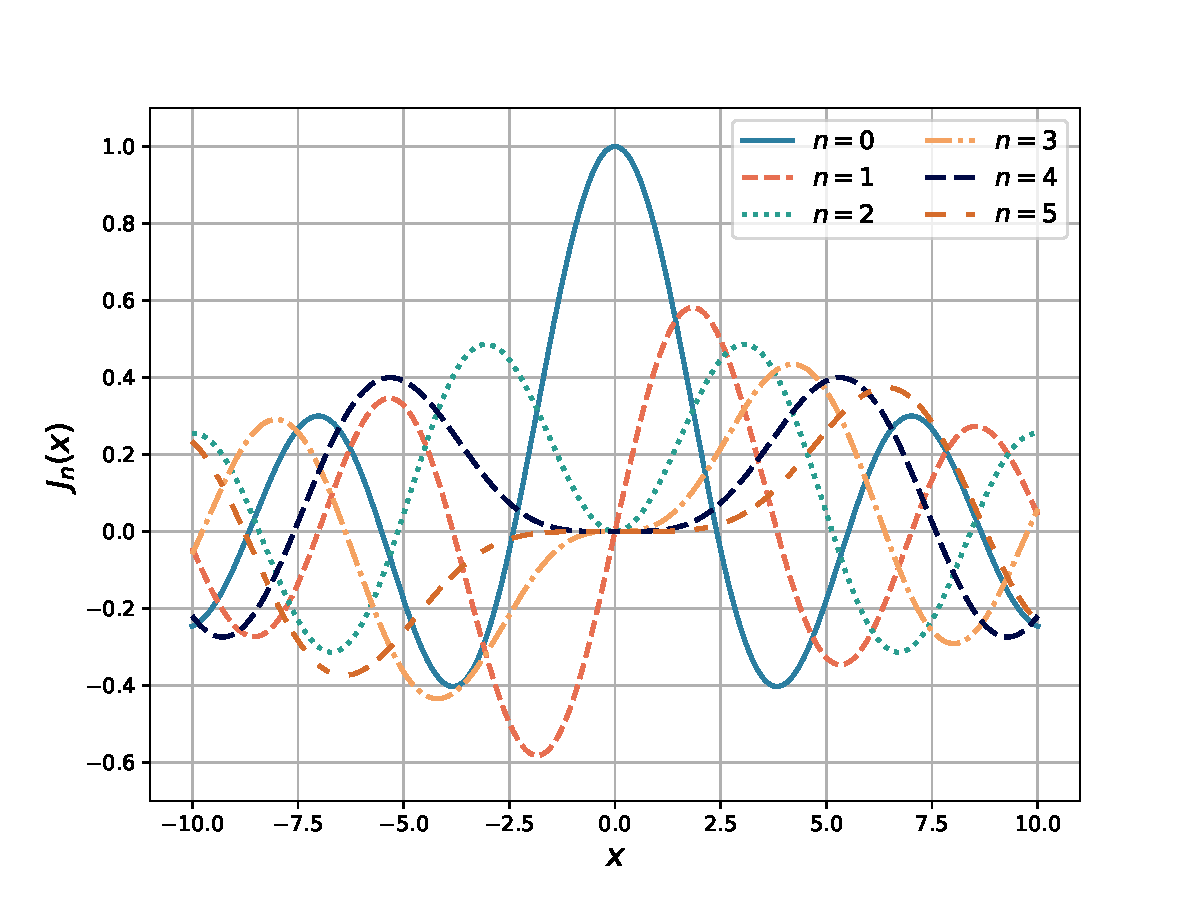
\includegraphics[width = 12cm]{Figuras/Bessel_first_Kind.pdf}
    \caption{Funciones de Bessel de orden entero para $n$ entre 0 y 5. Adaptación de \href{https://github.com/gfrubi/FM2/blob/master/figuras-editables/fig-Bessel.py}{este} código. La adaptación se encuentra \href{https://github.com/Pedroga-cc/Fisica-Matematica-II/blob/main/Figuras/Plotter_Bessel.py}{aquí}.}
    % \end{subfigure}
    %
    % \begin{subfigure}[b]{\textwidth}
    %     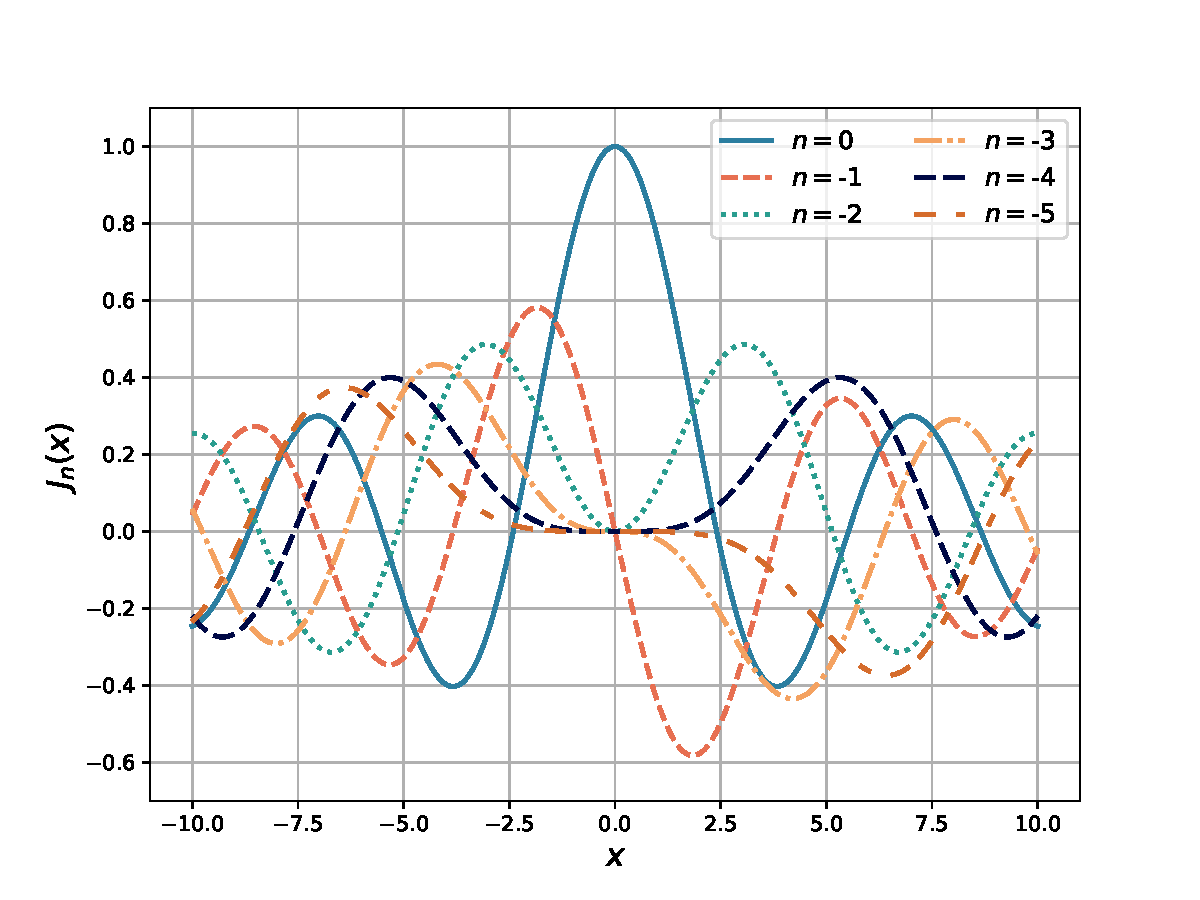
\includegraphics[width = 12cm]{Figuras/Bessel_first_Kind_negative.pdf}
    %     \caption{}
    % \end{subfigure}
    % \caption{aaa}
    \label{fig:Bessel_entero}
\end{figure}

\subsection{Funciones de Bessel de segunda especie, o de Neumann}

Mediante el método de Frobenius, podemos también encontrar soluciones logarítmicas. Mediante este método, podemos encontrar que una segunda solución de este tipo.

\begin{defi} \marginnote{Funciones de Bessel de segunda especie}
    Se denominan \textbf{funciones de Bessel de segunda especie} $Y_\nu(x)$, o \textbf{funciones de Neumann} $N_\nu(x)$ a las soluciones de tipo logarítmica obtenidas a partir del método de Frobenius para la EDO de Bessel \eqref{eq:EDO_Bessel}, linealmente independientes a $J_\nu(x)$.

    Alternativamente, las definimos más comúnmente como
    \begin{equation}
        Y_\nu(x) = N_\nu(x) = \frac{\cos(\pi \nu) J_\nu(x) - J_{-\nu(x)}}{\sin(\pi \nu)} \ , \qquad \nu \notin \mathbb{Z} \ .
    \end{equation}
\end{defi}
% denominada históricamente \textbf{funciones de Neumann} $N_\nu(x)$, o más recientemente \textbf{funciones de Bessel de segunda especie}, $Y_\nu(x)$, como
% \begin{equation}
%     Y_\nu(x) = N_\nu(x) = \frac{\cos(\pi \nu) J_\nu(x) - J_{-\nu(x)}}{\sin(\pi \nu)} \ , \qquad \nu \notin \mathbb{Z} \ ,
% \end{equation}
% que es linealmente independiente a $J_\nu(x)$.\footnote{No se aprecia directamente, pero las funciones de Bessel de segunda especie son soluciones de tipo logarítmicas. Aquí se prefiere utilizar la notación que involucra senos y cosenos por simplicidad, evitando escribir una solución en serie en cada momento.} 

En base a esta definición, podemos también escribir las soluciones generales de la ecuación de Bessel como
\begin{equation}
    y(x) = C_3 J_\nu(x) + C_4 Y_\nu(x) \ .
\end{equation}

La definición dada más arriba es válida para números \emph{no enteros}. Cuando deseamos trabajar con números enteros, es posible demostrar, usando la regla de L'Hôpital, que esta solución sigue siendo linealmente independiente en el límite en que $\nu \to n$, de modo que
\begin{equation}
    Y_n(x) = \lim_{\nu \to n} \frac{\cos(\pi \nu) J_\nu(x) - J_{-\nu(x)}}{\sin(\pi \nu)} \ , \qquad n \in \mathbb{Z} \ .
\end{equation}
Nótese que estas funciones divergen para $x = 0$, como se observa más claramente en la figura \ref{fig:Bessel_segunda_especie}.

De forma similar a las funciones de Bessel de primera especie, estas satisfacen, para orden entero, 
\begin{equation}
    Y_{-n}(x) = (-1)^n Y_n(x) \ .
\end{equation}

\begin{figure}
    \centering
    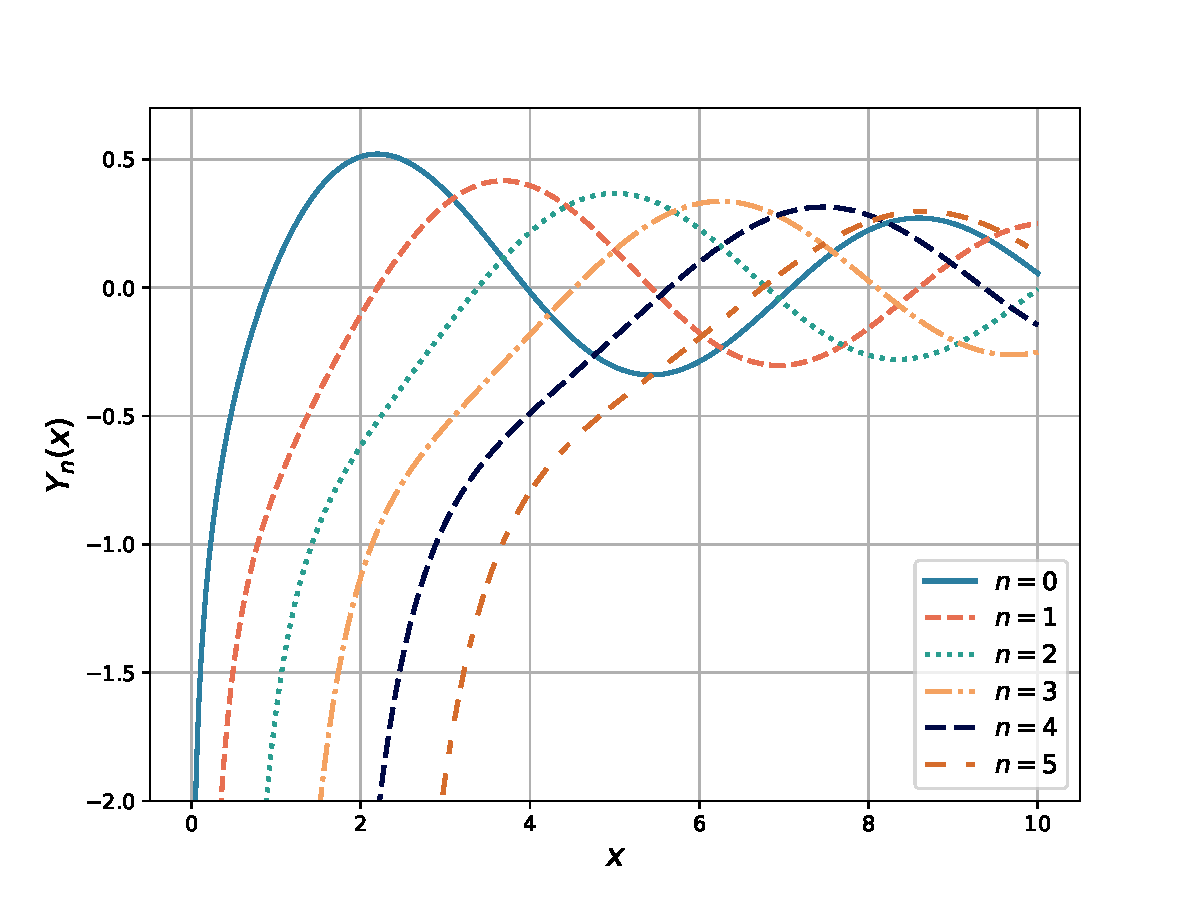
\includegraphics[width = 12cm]{Figuras/Bessel_second_kind.pdf}
    \caption{Funciones de Neumann de orden entero para $n$ entre 0 y 5. Adaptación de \href{https://github.com/gfrubi/FM2/blob/master/figuras-editables/fig-Bessel.py}{este} código. La adaptación se encuentra \href{https://github.com/Pedroga-cc/Fisica-Matematica-II/blob/main/Figuras/Plotter_Bessel.py}{aquí}.}
    \label{fig:Bessel_segunda_especie}
\end{figure}

\newpage

\subsection{Funciones de Hankel}

\begin{defi} \marginnote{Funciones de Hankel}
    Se definen las \textbf{funciones de Hankel} $H_\nu^{(1)}(x)$ y $H_\nu^{(2)}(x)$ como dos soluciones linealmente independientes para la EDO de Bessel \eqref{eq:EDO_Bessel}, dadas por
    \begin{align}
        H_\nu^{(1)}(x) & = J_\nu(x) + i Y_\nu(x) \ , \\
        H_\nu^{(2)}(x) & = J_\nu(x) - i Y_\nu(x) \ .
    \end{align}
\end{defi}

¿Por qué definimos otro tipo de soluciones a la EDO de Bessel? Pues es útil trabajar con funciones de Hankel al estudiar soluciones de la ecuación de onda, e históricamente ha sido la ruta a seguir. Además, mediante su representación integral (que mencionaremos más adelante), es posible mostrar\footnote{Puede encontrar el detalle en \cite{Arfken}, pues no considero relevante hacerlo aquí.} que las funciones de Hankel satisfacen las relaciones
\begin{align}
    H_\nu^{(1)}(x) & = e^{-i\nu\pi} H_{-\nu}^{(1)}(x) \ , \\
    H_\nu^{(2)}(x) & = e^{i\nu\pi} H_{-\nu}^{(2)}(x) \ .
\end{align}

% También es útil definir, particularmente al estudiar soluciones de la ecuación de onda, un nuevo conjunto de funciones linealmente independientes, las llamadas \textbf{funciones de Hankel}, que son combinaciones lineales de las funciones de Bessel y Neumann,
% \begin{align}
%     H_\nu^{(1)}(x) & = J_\nu(x) + Y_\nu(x) \ , \\
%     H_\nu^{(2)}(x) & = J_\nu(x) - Y_\nu(x) \ .
% \end{align}

% Mediante su representación integral (que mencionaremos más adelante), es posible mostrar\footnote{En este caso, el detalle puede encontrarse en \cite{Arfken}.} que las funciones de Hankel satisfacen las relaciones
% \begin{align}
%     H_\nu^{(1)}(x) = e^{-i\nu\pi} H_{-\nu}^{(1)}(x) \ , \\
%     H_\nu^{(2)}(x) = e^{i\nu\pi} H_{-\nu}^{(2)}(x) \ .
% \end{align}


\subsection{Función generatriz (para orden entero)}

En el caso en que $\nu$ es un número entero, podemos escribir una función generatriz de una forma análoga a cualquier polinomio ortogonal, a pesar de que las funciones de Bessel no son polinomios. En este caso, esta tiene la forma
\begin{equation}
    G(x,t) = \exp\left[ \frac{x}{2} \left( t - \frac{1}{t} \right) \right] = \sum_{n = -\infty}^\infty J_n(x) t^n \ .
\end{equation}
Es directo verificar la segunda igualdad al expandir la exponencial en una serie de potencias para $t$. Gracias a la función generatriz, podemos hallar de una forma más sencilla algunas propiedades para las funciones de Bessel de orden entero.

\subsection{Ceros de las funciones de Bessel}

Las funciones de Bessel son funciones oscilantes, pero no periódicas. Por ello, si bien tienen infinitos ceros (puntos para los cuales $J_\nu(x) = 0$), no existe una forma analítica de calcularlos. Por este motivo, estos valores son calculados de forma numérica a partir de, por ejemplo, la expresión en serie para las funciones de Bessel. Denotaremos la $n-$ésima raíz de la función de Bessel de orden $\nu$ como $\alpha_{\nu, n}$, tal que $J(\alpha_{\nu, n}) = 0$. Además, estas cumplen que $\alpha_{\nu, n+1} > \alpha_{\nu, n}$. Mostramos algunos ceros para funciones de orden entero en la tabla \ref{tab:alphanun}.

\begin{table}[htbp]
    \centering
    \begin{tabular}{ccccccc}
    \hline $\alpha_{\nu,n}$ & $n=1$ & $n=2$ & $n=3$ & $n=4$ & $n=5$ \\ \hline 
    $\nu=0$ & 2.4048255 &  5.5200781 &  8.6537279 & 11.7915344 & 14.9309177\\
    $\nu=1$ & 3.8317059 &  7.0155866 & 10.1734681 & 13.3236919 & 16.4706300\\
    $\nu=2$ & 5.1356223 &  8.4172441 & 11.6198411 & 14.7959517 & 17.9598194 \\
    $\nu=3$ & 6.3801619 &  9.7610231 & 13.0152007 & 16.2234661 & 19.4094152 \\
    $\nu=4$ & 7.5883424 & 11.0647094 & 14.3725366 & 17.6159660 & 20.8269329 \\
    \hline 
    \end{tabular} 
    \caption{Las primeras raíces $\alpha_{\nu,n}$ de $J_\nu(x)$, $\nu=0,1,2,3,4$. Un Código Python para hallarlas se encuentra disponible en \href{https://github.com/gfrubi/FM2/blob/master/Notebooks/Bessel-Ceros.ipynb}{este} notebook.}
    \label{tab:alphanun}
\end{table}

De igual manera, a veces es necesario utilizar los ceros de las derivadas de las funciones de Bessel, los que denotaremos por $\beta_{\nu, n}$. Ellos, al igual que los $\alpha_{\nu, n}$, satisfacen que $\beta_{\nu, n+1} > \beta_{\nu, n}$. Algunos valores numéricos se presentan en la tabla \ref{tab:betanun}.

\begin{table}[htbp]
    \centering
    \begin{tabular}{ccccccc}
    \hline $\beta_{m,n}$ & $n=1$ & $n=2$ & $n=3$ & $n=4$ & $n=5$ \\ \hline 
    $m=0$ & 3.8317059 &  7.0155866 & 10.1734681 & 13.3236919 & 16.4706300\\
    $m=1$ & 1.8411837 &  5.3314427 &  8.5363163 & 11.7060049 & 14.8635886 \\
    $m=2$ & 3.0542369 &  6.7061331 &  9.9694678 & 13.1703708 & 16.3475223 \\
    $m=3$ & 4.2011889 &  8.0152366 & 11.3459243 & 14.5858482 & 17.7887478 \\
    $m=4$ & 5.3175531 &  9.2823962 & 12.6819084 & 15.9641070 & 19.1960288 \\
    \hline 
    \end{tabular} 
    \caption{Las primeras raíces $\beta_{m,n}$ de $J'_m(x)$, $m=0,1,2,3,4$. Un Código Python para hallarlas se encuentra disponible en \href{https://github.com/gfrubi/FM2/blob/master/Notebooks/Bessel-Ceros.ipynb}{este} notebook.}
    \label{tab:betanun}
\end{table}


\subsection{Propiedades}
\begin{propiedad}
    \textbf{Propiedades de las funciones de Bessel}

    \begin{enumerate}
        % \item \textbf{Normalización.} Dada una raíz $\alpha_{\nu, n}$ de la función de Bessel de orden $\nu$, se satisface que
        % \begin{equation}
        %     \int_0^a r \left[J_\nu\left( \alpha_{\nu, n} \frac{x}{a} \right)\right]^2 dr = \frac{a^2}{2} \left[ J_{\nu+1}(\alpha_{\nu, n}) \right]^2 \ . 
        % \end{equation}
        \item \textbf{Ortogonalidad respecto a las raíces.} Para valores de $\nu$ no negativos, para $a > 0$ y para $n, m \in \mathbb{N}$, se tiene que
        \begin{equation}
            \int_0^a x J_{\nu} \left( \frac{\alpha_{\nu, n}}{a} x \right) J_\nu\left( \frac{\alpha_{\nu, m}}{a} x \right) dx = \frac{a^2}{2} [J'_\nu(\alpha_{\nu, n})]^2 \delta_{n, m} = \frac{a^2}{2} [J_{\nu+1}(\alpha_{\nu, n})]^2 \delta_{n, m} \ .
        \end{equation}
        Similarmente, para las raíces de la derivada de la función de Bessel, se tiene
        \begin{equation}
            \int_0^a x J_\nu\left(\frac{\beta_{\nu, n}}{a}x \right) J_\nu\left(\frac{\beta_{\nu, m}}{a}x \right) dx = \frac{a^2}{2} \left( 1 - \frac{\nu^2}{\beta^2_{\nu, n}} \right) \left[ J_\nu(\beta_{\nu, n}) \right]^2 \ .
        \end{equation}
        % 
        % En general, dadas dos constantes $u, v$, y dado el intervalo $[a,b]$, las funciones de Bessel satisfacen
        % \begin{equation}
        %     \int_a^b x J_\nu(u x) J_\nu(bx) dx = \frac{1}{u^2-v^2} \left[ vx J_\nu(ux) J0_\nu(vx) - ux J_\nu(vx) J'_\nu(ux) \right]_a^b \delta_{u,v} \ .
        % \end{equation} 
        \item \textbf{Ortogonalidad respecto al orden.} Las funciones de Bessel, en general, \emph{no son ortogonales respecto a los índices}, es decir, $\left\langle J_\mu(x), J_\nu(x) \right\rangle \neq 0$.
        \item \textbf{Completitud.} Las funciones de Bessel (de orden no negativo) forman un \emph{conjunto completo} de funciones en el intervalo $[0,a]$, lo que se puede representar aproximadamente como \cite{Reimberg2015}
        \begin{equation}
            \sum_{k=1}^\infty \frac{J_{\nu-1} \left(\frac{ \alpha_{\mu, k}}{a}x \right) J_{\nu-1} \left(\frac{\alpha_{\mu, k}}{a} y \right)}{\left[J_{\mu+1}(\alpha_{\mu, k})\right]^2} = \frac{a}{2x} \delta\left( \frac{x}{a} - \frac{y}{a} \right) \ ,
        \end{equation}
        donde $\mu + 1 \geq \nu$, y $\mu - \nu > 1$.
        % \begin{equation}
        %     \int_0^\infty x J_\nu(ux) J_\nu(vx) dx = \frac{1}{u} \delta(u-v) \ ,
        % \end{equation}
        % para cualquier $\nu > -1/2$.
        \item \textbf{Serie de Fourier-Bessel.} Dado que las funciones de Bessel forman una base en el intervalo $[0,a]$, podemos expandir cualquier función en una Serie de Fourier-Bessel, tal que
        \begin{equation}
            f(x) = \sum_{n=0}^\infty c_{\nu, n} \ J_\nu\left(\alpha_{\nu, n} \frac{x}{a}\right) \ ,
        \end{equation}
        donde
        \begin{equation}
            c_{\nu, n} = \frac{2}{a^2 \left[J_{\nu+1}(\alpha_{\nu, n})\right]^2} \int_0^a x f(x) \ J_\nu\left( \alpha_{\nu, k} \frac{x}{a} \right) dx \ .
        \end{equation}
        \item \textbf{Representación Integral.} Por motivos históricos, las funciones de Bessel fueron encontradas como soluciones a ecuaciones integrales. Por ello, listamos las representaciones integrales más comunes, que pueden ser obtenidas como una Serie de Laurent de la función generatriz.
        \begin{align}
            J_n(x) & = \frac{1}{\pi}\int_0^\pi \cos(nt - x\sin t) dt \ , \\
            J_\nu(x) & = \frac{1}{\pi} \int_0^\pi \cos(\nu t - x\sin t) dt - \frac{\sin(\nu \pi)}{\pi} \int_0^\infty e^{-x \sinh t - \nu t} dt \ , \\
            Y_n(x) & = \frac{1}{\pi} \int_0^\pi \sin(x\sin t - nt) dt - \frac{1}{\pi} \int_0^\infty \left[e^{nt} + (-1)^n e^{-nt} \right] e^{-x \sinh t} dt \ .
        \end{align}
    
        Gracias a ellas, podemos obtener tres resultados interesantes, los que son 
        \begin{align}
            \cos(x \sin \theta) & = J_0(x) + 2 \sum_{n*1}^\infty J_{2n}(x) \cos(2n\theta) \ , \\
            \sin(x \sin \theta) & = 2 \sum_{n=1}^\infty J_{2n-1}(x) \sin((2n-1)\theta) \ ,
        \end{align}
        y para el caso en que $\theta = 0$, 
        \begin{equation}
            J_0(x) + 2\sum_{n=1}^\infty J_{2n}(x) = 1 \ .
        \end{equation}
        \item \textbf{Comportamiento asintótico.} En el límite en que $x$ toma valores \emph{muy grandes}, generalmente entendido como $x \gg |\nu^2 - 1/4|$, podemos representar las funciones de Bessel como
        \begin{align}
            J_\nu(x) & \approx \sqrt{\frac{2}{\pi x}} \cos\left( x - \frac{\nu \pi}{2} - \frac{\pi}{4} \right) \ , \\
            Y_\nu(x) & \approx \sqrt{\frac{2}{\pi x}} \sin\left( x - \frac{\nu \pi}{2} - \frac{\pi}{4} \right) \ , \\
            H^{(1)}_\nu(x) = H^{(2)}_\nu(x)^\ast & = \sqrt{\frac{2}{\pi x}} \exp\left[ i \left( x - \frac{\nu \pi}{2} - \frac{\pi}{4} \right) \right] \ .
        \end{align}
        \item \textbf{Relaciones de Recurrencia.} Por definición, cualquier función de Bessel (incluyendo las de Neumann y de Hankel) debe satisfacer las siguientes relaciones de recurrencia:
        \begin{align}
            Z_{n+1}(x) + Z_{n-1}(x) & = \frac{2n}{x} Z_n(x) \ , \\
            Z_{n+1}(x) - Z_{n-1}(x) & = -2 Z'_n(x) \ . 
        \end{align}

        \item \textbf{Relaciones con derivadas.} A partir de las relaciones de recurrencia, es posible mostrar que cualquier función de Bessel satisface
        \begin{align}
            x^\nu Z_{\nu-1}(x) & = \frac{d}{dx}\left[ x^\nu Z_\nu(x) \right] \ , \\
            -x^{-\nu} Z_{\nu+1}(x) & = \frac{d}{dx}\left[ x^{-\nu} Z_\nu(x) \right] \ , \\
            \frac{d}{dx} \left[ Z_\nu(x) \right] & = \frac{1}{2} \left[ Z_{\nu-1}(x) - Z_{\nu+1}(x) \right] \ .
        \end{align}
    \end{enumerate}
\end{propiedad}


\section{Funciones modificadas de Bessel}

¿Qué pasaría si, en la ecuación \eqref{eq:EDO_Bessel}, $x^2$ tuviera signo negativo en lugar de positivo? Es decir, si la ecuación toma la forma
\begin{equation}\label{eq:Bessel_modificada}
    x^2 \frac{d^2y}{dx^2} + x \frac{dy}{dx} - (x^2 + \nu^2)y = 0 \ . 
\end{equation}

Esta ecuación es conocida como la \textbf{ecuación modificada de Bessel}, y sus soluciones, a diferencia de las funciones de Bessel, \emph{no son oscilantes}, sino que su comportamiento es exponencial. Por suerte, métodos análogos a los utilizados anteriormente nos permiten encontrar soluciones a esta ecuación.

\begin{defi} \marginnote{Funciones modificadas de Bessel}
    Un conjunto particular de soluciones a la ecuación modificada de Bessel \eqref{eq:Bessel_modificada} corresponde a las \textbf{funciones modificadas de Bessel de primera especie}, $I_\nu(x)$, y a las \textbf{funciones modificadas de Bessel de segunda especie}, $K_\nu(x)$, definidas como
    \begin{align}
        I_\nu(x) & = i^{-\nu} J_\nu(ix) = \sum_{k=0^\infty} \frac{1}{k! \Gamma(k+\nu+1)} \left( \frac{x}{2} \right)^{2k+\nu} \ , \\
        K_\nu(x) & = i^{\nu + 1} \frac{\pi}{2} H_\nu^{(1)}(ix) = \frac{\pi}{2} \left[ \frac{I_{-\nu}(x) - I_\nu(x)}{\sin(\nu \pi)} \right] \ , \qquad \nu \notin \mathbb{Z} \ .
    \end{align}
\end{defi}

De forma análoga a lo ocurrido para las funciones de Bessel de segunda especie, en caso en que $\nu$ sea entero, las funciones modificadas de segunda especie se definen como el límite
\begin{equation}
    K_n(x) = \lim_{\nu \to n} \frac{\pi}{2} \left[ \frac{I_{-\nu}(x) - I_\nu(x)}{\sin(\nu \pi)} \right] \ , \qquad n \in \mathbb{Z} \ .
\end{equation}

\begin{figure}[htbp]
    \centering
    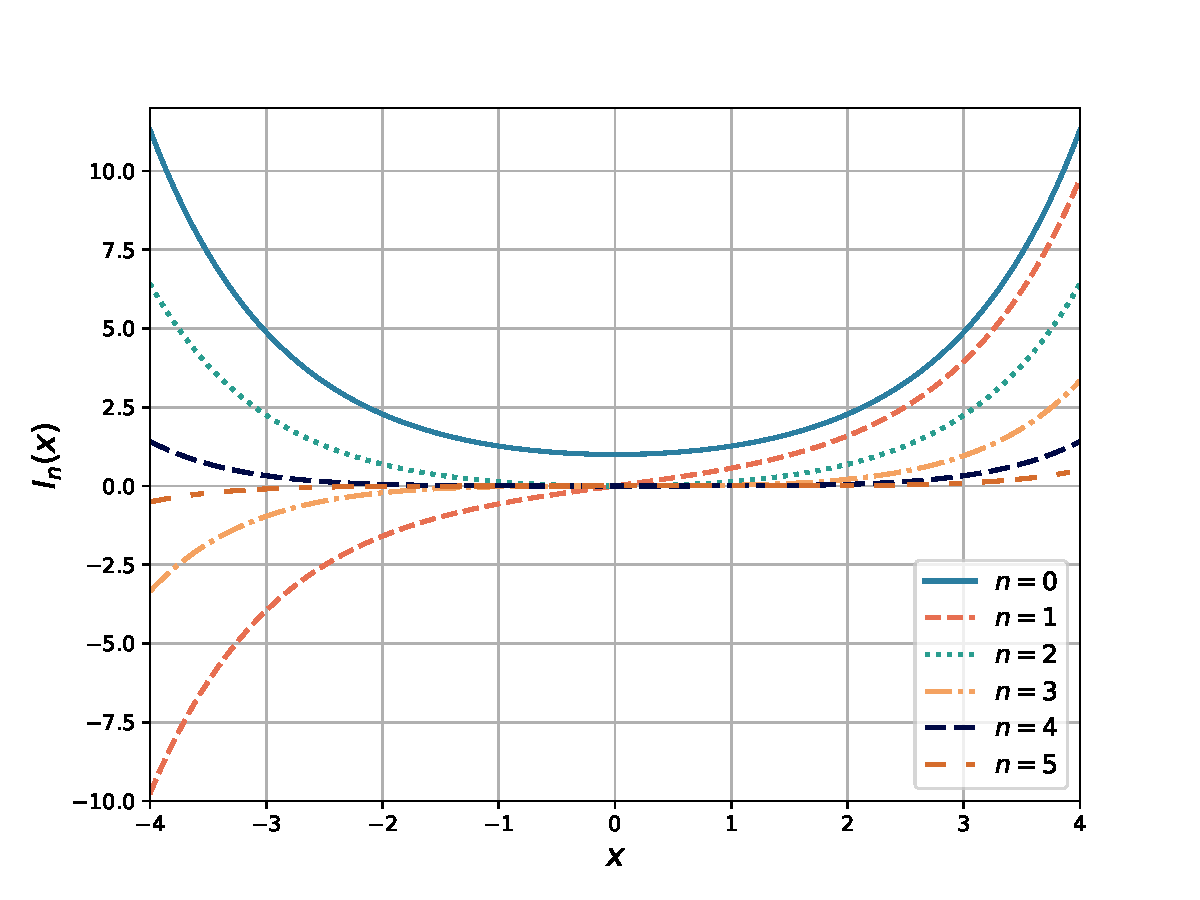
\includegraphics[width = 10cm]{Figuras/Bessel-modified-first-kind.pdf}
    \caption{Funciones de Bessel modificadas de primera especie. Figura adaptada a partir de \href{https://github.com/gfrubi/FM2/blob/master/figuras-editables/fig-Bessel.py}{este} código. La adaptación se encuentra \href{https://github.com/Pedroga-cc/Fisica-Matematica-II/blob/main/Figuras/Plotter_Bessel.py}{aquí}.}
    \label{fig:Bessel_modificada_primera}
\end{figure}

\begin{figure}[htbp]
    \centering
    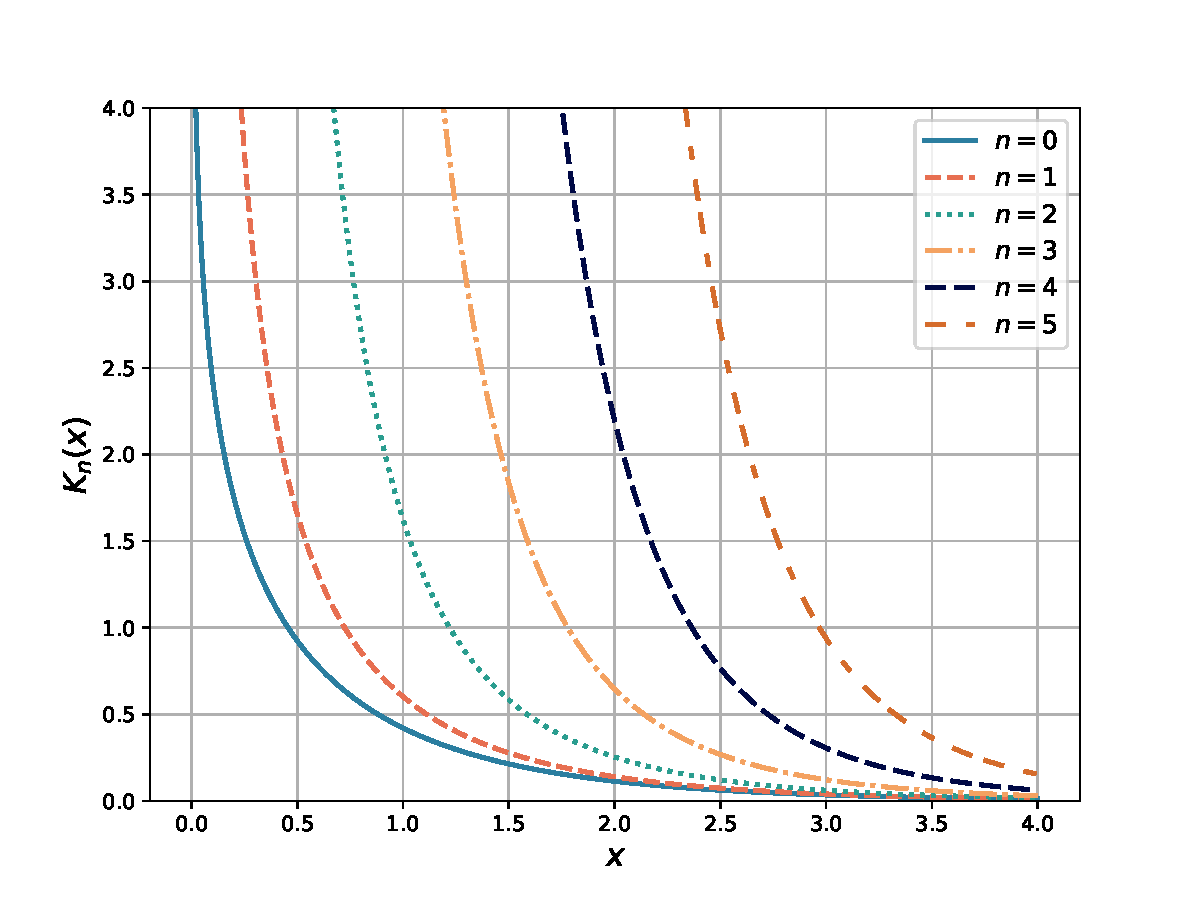
\includegraphics[width = 10cm]{Figuras/Bessel-modified-second-kind.pdf}
    \caption{Funciones de Bessel modificadas de segunda especie. Figura adaptada a partir de \href{https://github.com/gfrubi/FM2/blob/master/figuras-editables/fig-Bessel.py}{este} código. La adaptación se encuentra \href{https://github.com/Pedroga-cc/Fisica-Matematica-II/blob/main/Figuras/Plotter_Bessel.py}{aquí}.}
    \label{fig:Bessel_modificada_segunda}
\end{figure}

% \begin{figure}[htbp]
%     \centering
%     \begin{subfigure}{\textwidth}
%         \centering
%         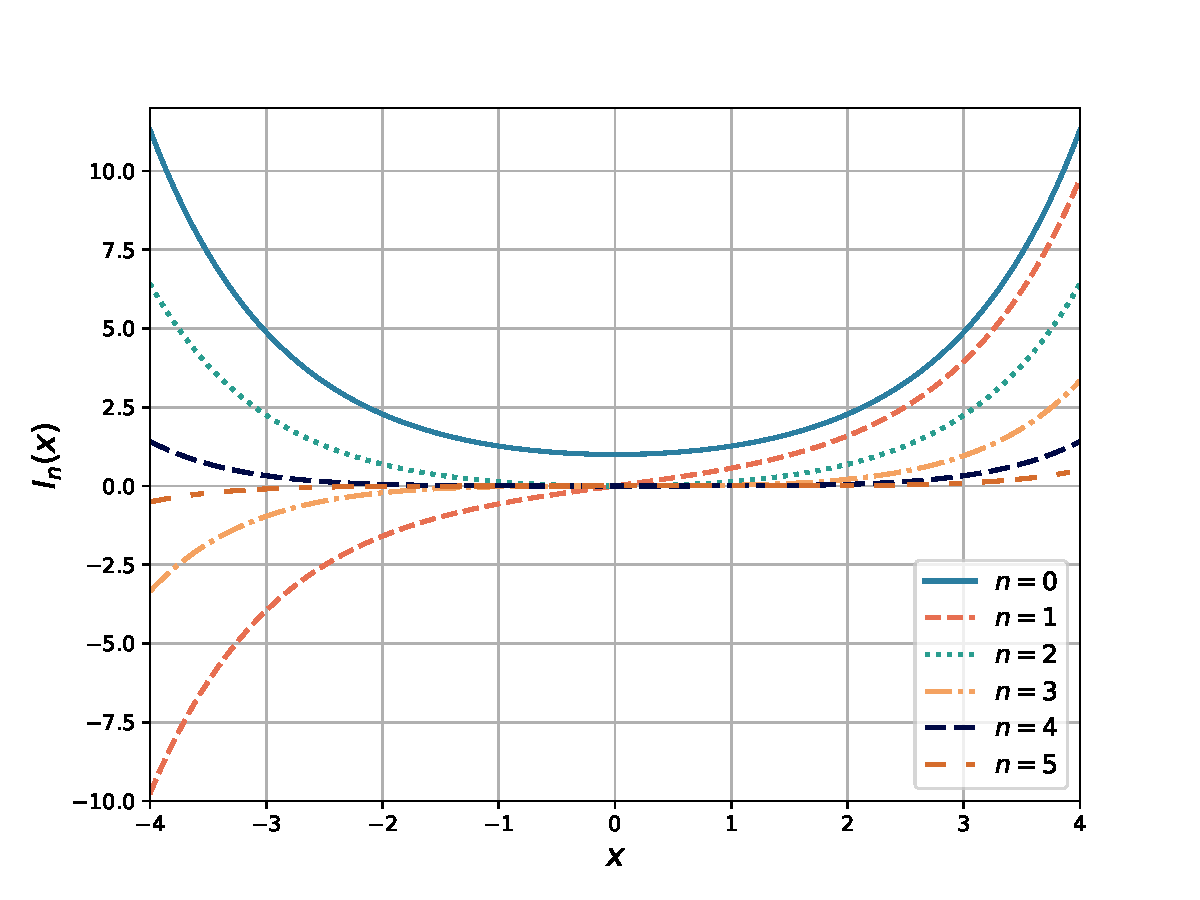
\includegraphics[width = 10cm]{Figuras/Bessel-modified-first-kind.pdf}
%         \caption{\label{fig:Bessel_modificada_primera}}
%     \end{subfigure}
%     \begin{subfigure}{\textwidth}
%         \centering
%         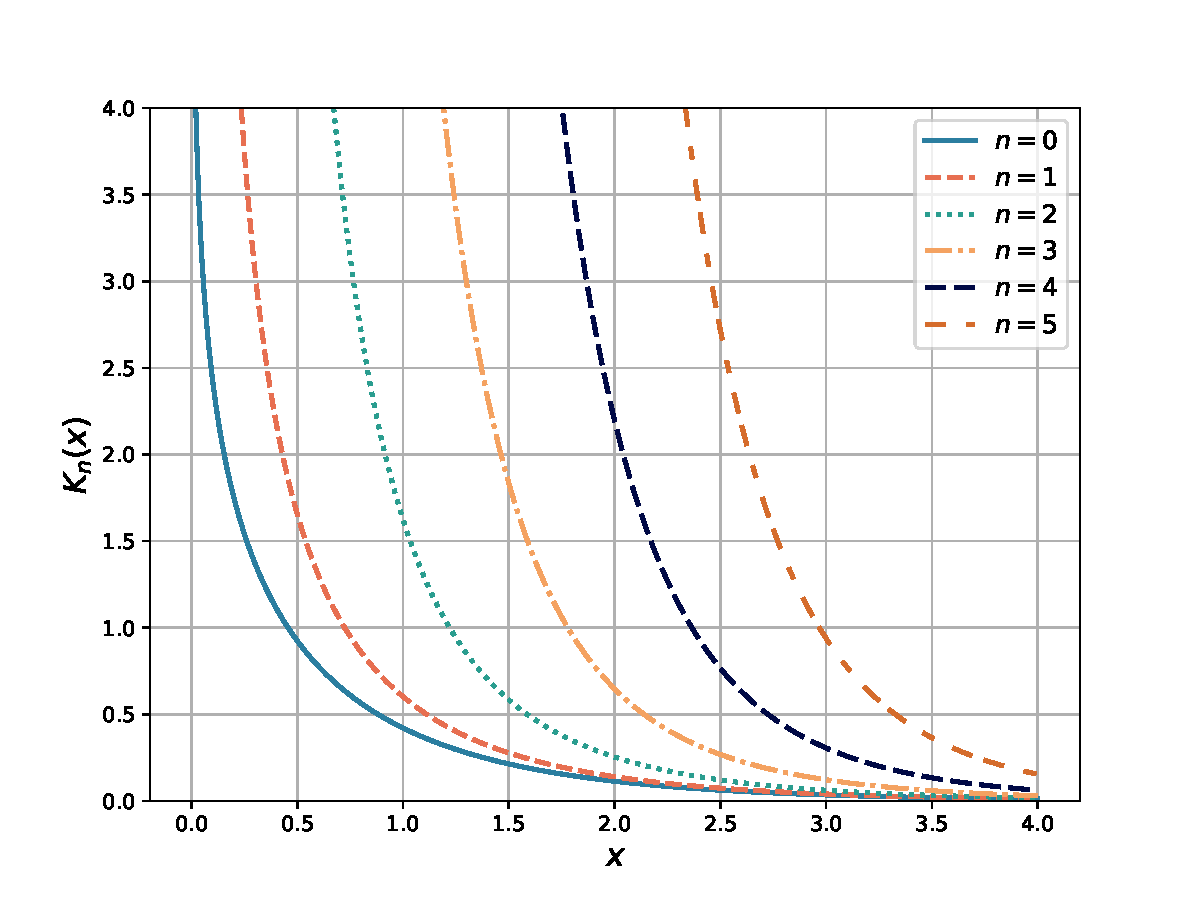
\includegraphics[width = 10cm]{Figuras/Bessel-modified-second-kind.pdf}
%         \caption{\label{fig:Bessel_modificada_segunda}}
%     \end{subfigure}
%     \caption{Funciones de Bessel modificadas de \subref{fig:Bessel_modificada_primera} primera especie y \subref{fig:Bessel_modificada_segunda} segunda especie. Figura adaptada a partir de \href{https://github.com/gfrubi/FM2/blob/master/figuras-editables/fig-Bessel.py}{este} código. La adaptación se encuentra \href{aa}{aquí}.}
%     \label{fig:Bessel_modificada}
% \end{figure}

\subsection{Propiedades}

\begin{propiedad}
    \textbf{Propiedades de las funciones modificadas de Bessel.}

    \begin{enumerate}
        \item \textbf{Comportamiento asintótico.} En el límite en que $x$ toma valores \emph{muy grandes}, generalmente entendido como $x \gg |\nu^2 - 1/4|$, podemos representar las funciones de Bessel como
        \begin{align}
            I_\nu(x) & = \frac{1}{\sqrt{2\pi x}} e^x \ , \\
            K_\nu(x) & = \sqrt{\frac{\pi}{2x}} e^{-x} \ . 
        \end{align}
        \item \textbf{Relaciones de recurrencia.} Las funciones modificadas de Bessel satisfacen las siguientes relaciones de recurrencia,
        \begin{align}
            I_{\nu - 1}(x) - I_{\nu + 1}(x) & =   \frac{2\nu}{x} I_\nu(x) \ , \\
            K_{\nu - 1}(x) - K_{\nu + 1}(x) & = - \frac{2\nu}{x} K_\nu(x) \ , \\
            I_{\nu - 1}(x) + I_{\nu + 1}(x) & =   2 I'_\nu(x) \ , \\
            K_{\nu - 1}(x) + K_{\nu + 1}(x) & = - 2 K'_\nu(x) \ .
        \end{align}
        \item \textbf{Relaciones con derivadas.} A partir de las relaciones de recurrencia, podemos hallar las relaciones
        \begin{align}
            x^{\nu} I_{\nu - 1}(x)    & = \frac{d}{dx}[x^\nu    I_\nu(x)] \ , \\
            - x^{\nu} K_{\nu - 1}(x)  & = \frac{d}{dx}[x^\nu    K_\nu(x)] \ , \\
            x^{-\nu} I_{\nu + 1}(x)   & = \frac{d}{dx}[x^{-\nu} I_\nu(x)] \ , \\
            - x^{-\nu} K_{\nu + 1}(x) & = \frac{d}{dx}[x^{-\nu} K_\nu(x)] \ .
        \end{align}
    \end{enumerate}
\end{propiedad}

\begin{ejemplo}
    \textbf{(Butkov, sección 9.11.)} Considere un cilindro circular sólido de radio $b$ y longitud $L$. Las bases del cilindro se mantienen a temperatura cero, $u(z = 0, t) = u(z = L, t) = 0$, mientras que su superficie lateral es mantenida a una temperatura $u(\rho = b, t) = T_1$ constante. Encuentre la distribución de temperatura en el interior del cilindro en el estado estacionario.

    \textbf{Solución.} Cuando nos referimos a \emph{estado estacionario}, nos referimos al caso en que la temperatura se mantenga constante en el tiempo. Dado este requisito, la ecuación de difusión del calor se convertirá en la ecuación de Laplace, pues
    \begin{equation*}
        \nabla^2 u = \frac{1}{\alpha^2} \cancelto{0}{\frac{\partial u}{\partial t}} = 0 \ .
    \end{equation*}
    Dado que el sistema es un cilindro, también imponemos la condición de periodicidad sobre la variable angular, es decir, $u(\rho, \phi, z) = u(\rho, \phi + 2\pi, z)$. Realizando separación de variables, tendremos las ecuaciones
    \begin{align*}
        \frac{d^2 Z}{dz^2} & = \lambda_1 Z \ , \\
        \frac{d^2 \Phi}{d\phi^2} & = \lambda_2 \Phi \ , \\
        \frac{d}{d\rho}\left( \rho \frac{dP}{d\rho} \right) + \left[ \rho \lambda_1 + \frac{\lambda_2}{\rho} \right] & = 0 \ .
    \end{align*} 
    Imponiendo nuestras condiciones de contorno, concluimos que $\lambda_1 = -n^2 \pi^2/L^2$ para $n = 1, 2, 3, \dots$ (solución oscilante), y $\lambda_2 = -m^2$ para $m = 0, 1, 2, \dots$ Así, la ecuación para $P$ se convierte en
    \begin{equation*}
        \frac{d}{d\rho}\left( \rho \frac{dP}{d\rho} \right) - \left[ \rho \frac{n^2\pi^2}{L^2} + \frac{m^2}{\rho} \right] = 0 \ ,
    \end{equation*} 
    lo que corresponde a la EDO modificada de Bessel. Esto se aprecia de forma más clara bajo el cambio de variable $x = n\pi \rho/L$, $P(\rho) = y(x)$, donde tendremos
    \begin{equation*}
        x^2 \frac{d^2 y}{dy^2} + x \frac{dy}{dx} - (x^2 + m^2)y = 0 \ .
    \end{equation*}

    Esta EDO tiene por solución general a las funciones modificadas de Bessel, tal que
    \begin{equation*}
        P_{mn}(\rho) = A_{mn} I_m\left( \frac{n\pi \rho}{L} \right) + B_{mn} K_m\left( \frac{n\pi \rho}{L} \right) \ .
    \end{equation*}

    Ahora, dado que trabajamos con un cilindro de radio finito, $\rho \to \infty$ no es parte de nuestro dominio, por lo que la función $I_m(x)$ está definida para nuestro problema. En cambio, dado que $\rho = 0$ es parte de nuestro dominio, y la función $K_m(x)$ diverge para $x = 0$, descartamos esta solución imponiendo que $B_{mn} = 0$.

    Por otro lado, dado que nuestro sistema posee simetría axial como consecuencia de la condición de contorno $u(\rho = b) = T_1$, pues este valor es válido para cualquier valor de $\phi$, podemos concluir que basta con considerar el caso en que $m=0$, de modo que la solución para $P(\rho)$ es dada por
    \begin{equation*}
        P_n(\rho) = A_n I_0\left( \frac{n \pi \rho}{L} \right) \ ,
    \end{equation*}
    mientras que la solución general al problema es de la forma
    \begin{equation*}
        u(\rho, \phi, z) = \sum_{n=1}^\infty A_n \sin\left( \frac{n \pi z}{L} \right) I_0 \left( \frac{n \pi \rho}{L} \right) \ ,
    \end{equation*}
    donde el coeficiente $A_n$ se obtiene imponiendo la condición de contorno $u(\rho = b) = T_1$. Queda como ejercicio para el lector comprobar que luego de imponer la condición de contorno, la solución a nuestro problema será
    \begin{equation*}
        u(\rho, \phi, z) = \frac{4T_1}{\pi} \sum_{n=1, 3, 5, \dots}^\infty \frac{1}{n} \frac{I_0(n \pi \rho/L) \sin(n \pi z/L)}{I_0(n \pi b/L)} \ .
    \end{equation*}
\end{ejemplo}

% las que corresponden a las \textbf{funciones modificadas de Bessel de primera especie}, $I_\nu(x)$, y a las \textbf{funciones modificadas de Bessel de segunda especie}, $K_\nu(x)$, definidas como
% \begin{align}
%     I_\nu(x) & = i^{-\nu} J_\nu(ix) = \sum_{k=0^\infty} \frac{1}{k! \Gamma(k+\nu+1)} \left( \frac{x}{2} \right)^{2k+\nu} \ , \\
%     K_\nu(x) & = \frac{\pi}{2} \left[ \frac{I_{-\nu}(x) - I_\nu(x)}{\sin(\nu \pi)} \right] \ , \qquad \nu \notin \mathbb{Z} \ , \\
%     K_n(x) & = \lim_{\nu \to n} \frac{\pi}{2} \left[ \frac{I_{-\nu}(x) - I_\nu(x)}{\sin(\nu \pi)} \right] \ , \qquad n \in \mathbb{Z} \ .
% \end{align}

\section{Funciones esféricas de Bessel}

Hemos discutido que las funciones de Bessel surgen como solución de la \emph{EDO radial} que surge de separar la ecuación de Helmholtz para coordenadas cilíndricas, que denominamos EDO de Bessel. De manera análoga, la EDO radial que surge en coordenadas esféricas es denominada \textbf{ecuación esférica de Bessel}, y es dada por
\begin{equation}
    x^2 \frac{d^2y}{dx^2} + 2x \frac{dy}{dx} + (x^2 - \ell(\ell+1))y = 0 \ ,
\end{equation}
donde hemos realizado el cambio de variables $x = kr$.

% Si bien las incluímos en el mismo capítulo dado su nombre, las \textbf{funciones esféricas de Bessel} surgen como soluciones de la parte radial de la ecuación de Helmholtz \emph{en coordenadas esféricas}, donde en la ecuación X hallamos que la ecuación esférica de Bessel es
% \begin{equation}
%     r^2 \frac{d^2R}{dr^2} + 2r \frac{dR}{dr} + [k^2 r^2 - \ell (\ell+1)]R(r) = 0 \ ,
% \end{equation}
% donde $\ell$ es un número entero. 
Notemos que, bajo la sustitución $y(x) = x^{-1/2} S(x)$, la ecuación toma la forma
\begin{equation} \label{eq:EDO_esferica_Bessel}
    x^2 \frac{d^2 S}{dx^2} + x \frac{dS}{dx} + \left[x^2 - \left(\ell + \frac{1}{2}\right)^2\right]S = 0 \ ,
\end{equation}
que al comparar con \eqref{eq:EDO_Bessel}, notamos que corresponde a la ecuación de Bessel de orden $\ell + 1/2$. Por ello, una solución de esta ecuación será
\begin{equation}
    y(x) = C_1 \frac{J_{\ell + 1/2}(x)}{\sqrt{x}} + C_2 \frac{Y_{\ell + 1/2}(x)}{\sqrt{x}} \ ,
\end{equation}
donde las constantes $C_1$ y $C_2$ se determinan a partir de las condiciones de contorno. En particular, cuando deseamos soluciones que sean finitas en el origen, escogeremos $C_2 = 0$.

\begin{defi} \marginnote{Funciones esféricas de Bessel}
    Las \textbf{funciones esféricas de Bessel} de primera y segunda especie corresponden a las soluciones de la ecuación esférica de Bessel \eqref{eq:EDO_esferica_Bessel} dadas por
    \begin{align}
        j_\ell(x) & = \sqrt{\frac{\pi}{2x}} J_{\ell + 1/2}(x) \ , \\
        y_\ell(x) = n_\ell(x) & = \sqrt{\frac{\pi}{2x}} Y_{\ell + 1/2}(x) \ .
    \end{align}
\end{defi}

% Bajo una normalización adecuada, preferimos definir las \textbf{funciones esféricas de Bessel} de primera y segunda especie como
% \begin{align}
%     j_\ell (x) & = \sqrt{\frac{\pi}{2x}} J_{\ell + 1/2}(x) \ , \\
%     y_\ell (x) = n_\ell(x) & = \sqrt{\frac{\pi}{2x}} Y_{\ell + 1/2} \ ,
% \end{align}
% donde, para $\ell$ entero, $Y_{\ell + 1/2}(x) = (-1)^{\ell + 1}J_{-\ell - 1/2}(x)$. 
Vale la pena hacer notar que
\begin{align}
    j_0(x) & = \frac{\sin x}{x} \ , \\
    y_0(x) & = - \frac{\cos x}{x} \ .
\end{align}
Además, cuando $\ell$ corresponde a un número entero, las funciones esféricas de Bessel satisfacen que
\begin{equation}
    y_{\ell+1/2}(x) = (-1)^{\ell+1} j_{-\ell - 1/2}(x) \ ,
\end{equation}
lo que es consecuencia de su relación con las funciones de Bessel de orden semientero.

\begin{figure}[htbp]
    \centering
    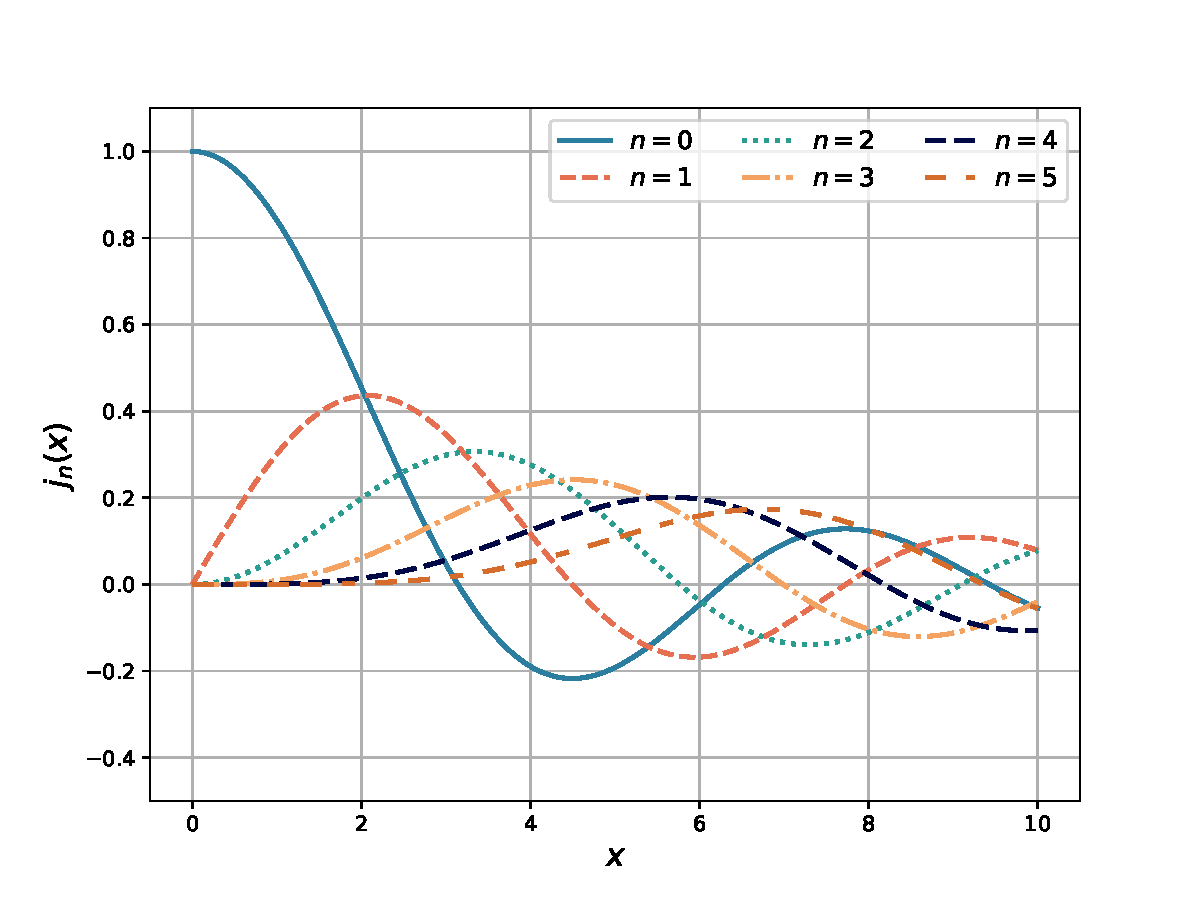
\includegraphics[width = 12cm]{Figuras/Bessel-Esferica-first-kind.pdf}
    \caption{Funciones esféricas de Bessel de orden entero para $n$ entre 0 y 5. Adaptación de \href{https://github.com/gfrubi/FM2/blob/master/figuras-editables/fig-Bessel.py}{este} código. La adaptación se encuentra \href{https://github.com/Pedroga-cc/Fisica-Matematica-II/blob/main/Figuras/Plotter_Bessel.py}{aquí}.}
    \label{fig:esferica_bessel_primera}
\end{figure}

\begin{figure}[htbp]
    \centering
    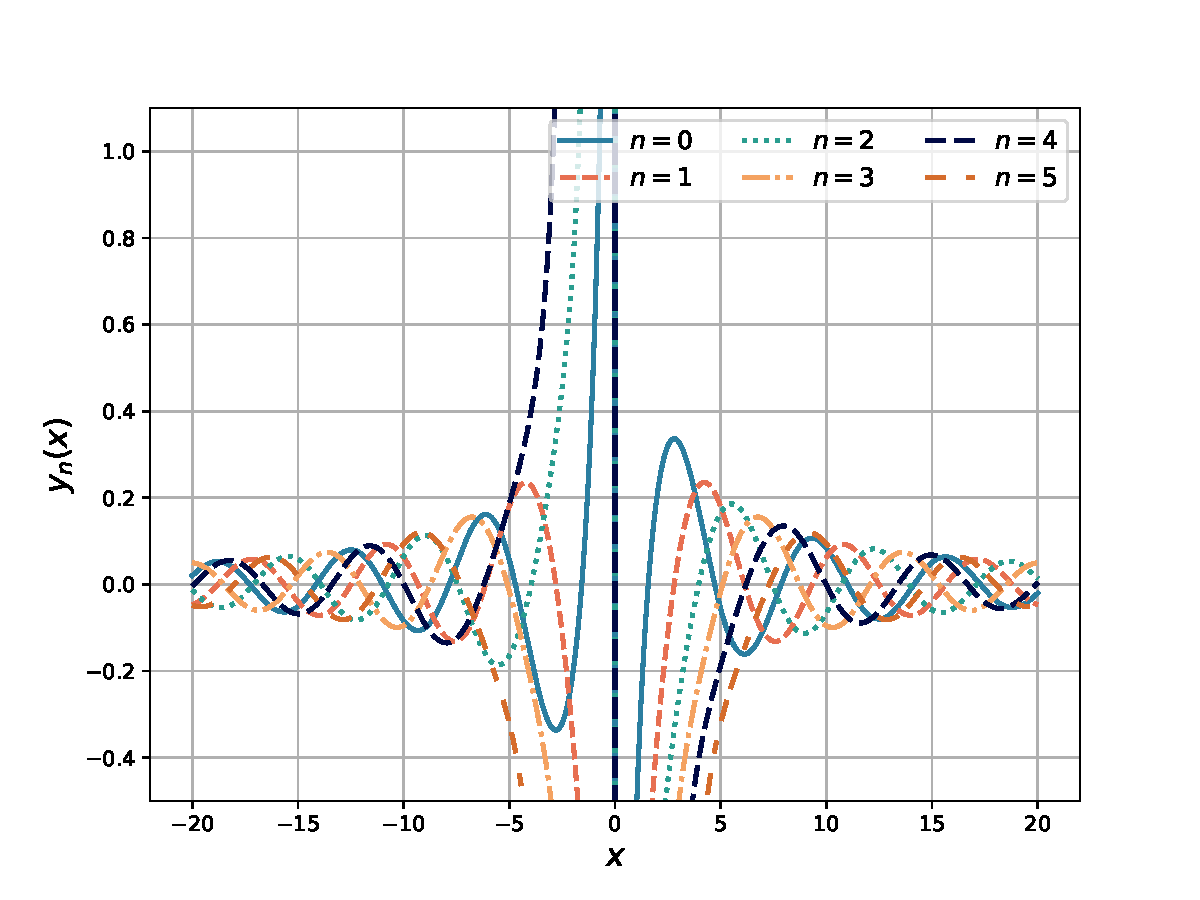
\includegraphics[width = 12cm]{Figuras/Bessel-Esferica-second-kind.pdf}
    \caption{Funciones esféricas de Neumann de orden entero para $n$ entre 0 y 5. Adaptación de \href{https://github.com/gfrubi/FM2/blob/master/figuras-editables/fig-Bessel.py}{este} código. La adaptación se encuentra \href{https://github.com/Pedroga-cc/Fisica-Matematica-II/blob/main/Figuras/Plotter_Bessel.py}{aquí}.}
    \label{fig:esferica_bessel_segunda}
\end{figure}

\subsection{Función generatriz (para orden entero)}

Las funciones esféricas de Bessel de orden entero pueden obtenerse a partir de las siguientes funciones generatrices
\begin{align}
    G_j(x,t) & = \frac{1}{x} \cos \left( \sqrt{x^2 - 2xt} \right) = \sum_{n=0}^\infty \frac{t^n}{n!} j_{n-1}(x) \ , \\
    G_y(x,t) & = \frac{1}{x} \sin \left( \sqrt{x^2 - 2xt} \right) = \sum_{n=0}^\infty \frac{t^n}{n!} y_{n-1}(x) \ .
\end{align} 

\subsection{Ceros de las funciones esféricas de Bessel}

Al igual que en el caso de las funciones de Bessel, no es posible hallar las raíces de las funciones esféricas de Bessel de forma analítica, por lo que en la tabla \ref{tab:alphanun_esferica} presentamos algunos ceros para funciones de orden entero. A su vez, en la tabla \ref{tab:betanun_esferica} presentamos los ceros de su primera derivada.

\begin{table}[htbp]
    \centering
    \begin{tabular}{ccccccc}
    \hline $\alpha_{n,p}$ & $n=1$ & $n=2$ & $n=3$ & $n=4$ & $n=5$ \\ \hline 
    $\nu=0$ & 3.1416 &  6.2832 &  9.4248 & 12.5664 & 15.7080 \\
    $\nu=1$ & 4.4934 &  7.7253 & 10.9041 & 14.0662 & 17.2208 \\
    $\nu=2$ & 5.7635 &  9.0950 & 12.3229 & 15.5146 & 18.6890 \\
    $\nu=3$ & 6.9879 & 10.4171 & 13.6980 & 16.9236 & 20.1218 \\
    $\nu=4$ & 8.1826 & 11.7049 & 15.0397 & 18.3013 & 21.5254 \\
    \hline 
    \end{tabular} 
    \caption{Las primeras raíces $\alpha_{n,p}$ de $j_n(x)$, $n=0,1,2,3,4$. Valores tomados del capítulo 14 de \cite{Arfken}.}
    \label{tab:alphanun_esferica}
\end{table}

\begin{table}[htbp]
    \centering
    \begin{tabular}{ccccccc}
    \hline $\beta_{n,p}$ & $n=1$ & $n=2$ & $n=3$ & $n=4$ & $n=5$ \\ \hline 
    $\nu=0$ & 4.4934 & 7.7253 & 10.9041 & 14.0662 & 17.2208 \\
    $\nu=1$ & 2.0816 & 5.9404 &  9.2058 & 12.4044 & 15.5792 \\
    $\nu=2$ & 3.3421 & 7.2899 & 10.6139 & 13.8461 & 17.0429 \\
    $\nu=3$ & 4.5141 & 8.5838 & 11.9727 & 15.2445 & 18.4681 \\
    $\nu=4$ & 5.6467 & 9.8404 & 13.2956 & 16.6093 & 19.8624 \\
    \hline 
    \end{tabular} 
    \caption{Las primeras raíces $\beta_{n,p}$ de $j'_n(x)$, $n=0,1,2,3,4$. Valores tomados del capítulo 14 de \cite{Arfken}.}
    \label{tab:betanun_esferica}
\end{table}

\subsection{Propiedades}

\begin{propiedad}
    \textbf{Propiedades de las funciones esféricas de Bessel.}

    \begin{enumerate}
        \item \textbf{Ortogonalidad respecto a las raíces.} A partir de la ortogonalidad de las funciones de Bessel, tenemos que
        \begin{equation}
            \int_0^a j_n\left( \alpha_{n,p} \frac{x}{a} \right) j_n\left( \alpha_{n,q} \frac{x}{a}  \right) r^2 \ dr = \frac{a^3}{2} \left[ j_{n+1}(\alpha_{np}) \right]^2 \delta_{pq} \ .
        \end{equation}
        \item \textbf{Ortogonalidad respecto al orden.} Tenemos que, a diferencia de las funciones de Bessel, las funciones esféricas de Bessel son ortogonales respecto a su orden, tal que
        \begin{equation}
            \int_{-\infty}^{+\infty} j_m(x) j_n(x) dx = \frac{\pi}{2n+1} \delta_{mn} \ .
        \end{equation}
        \item \textbf{Funciones esféricas de Hankel.} De forma análoga a las funciones de Bessel, podemos definir las funciones esféricas de Hankel como
        \begin{align}
            h_\ell^{(1)}(x) & = \sqrt{\frac{\pi}{2x}}H_{\ell + 1/2}^{(1)}(x) = j_n(x) + i y_n(x) \ , \\
            h_\ell^{(2)}(x) & = \sqrt{\frac{\pi}{2x}}H_{\ell + 1/2}^{(2)}(x) = j_n(x) - i y_n(x) \ .
        \end{align}
        \item \textbf{Expansión en serie de potencias.} Para el caso de orden entero, es posible representar las funciones esféricas de Bessel en términos de una serie de potencias, donde
        \begin{align}
            j_n(x) & = 2^n x^n  \sum_{k=0}^\infty \frac{(-1)^k}{k!} \frac{(k+n)!}{(2k+2n+1)!}x^{2k} \ , \\
            y_n(x) & = \frac{(-1)^{n+1}}{2^n x^{n+1}} \sum_{k = 0}^\infty \frac{(-1)^k (k-n)!}{k! (2k-2n)!}z^{2k} \ .
        \end{align}
        \item \textbf{Comportamiento asintótico.} A partir del comportamiento asintótico de las funciones de Bessel, tenemos que
        \begin{align}
            j_n(x) & \approx \frac{1}{x} \sin\left( x - \frac{n\pi}{2} \right) \ , \\
            y_n(x) & \approx - \frac{1}{x} \cos\left( x - \frac{n\pi}{2} \right) \ , \\
            h_n^{(1)}(x) = H_n^{(2)}(x)^\ast & = \approx (-i)^{n+1} \frac{e^{ix}}{x} = - \frac{e^{i(x-n\pi/2)}}{x} \ .
        \end{align}
        \item \textbf{Relaciones de recurrencia.} Cualquier función esférica de Bessel satisface las relaciones de recurrencia
        \begin{align}
            f_{n-1}(x) + f_{n+1}(x) & = \frac{2n+1}{x} f_n(x) \ , \\
            n f_{n-1}(x) - (n+1) f_{n+1}(x) & = (2n+1) f'_n(x) \ .
        \end{align}
        \item \textbf{Relaciones con derivadas.} Las funciones esféricas de Bessel de orden $n$ pueden obtenerse a partir de las funciones de orden 0 mediante sucesivas derivaciones, esto es,
        \begin{align}
            j_n(x) & = (-1)^n x^n \left( \frac{1}{x} \frac{d}{dx} \right)^n \left( \frac{\sin x}{x} \right) \ , \\
            y_n(x) & = (-1)^n x^n \left( \frac{1}{x} \frac{d}{dx} \right)^n \left( \frac{\cos x}{x} \right) \ , \\
            h_n^{(1)}(x) & = -i (-1)^n x^n \left( \frac{1}{x} \frac{d}{dx} \right)^n \left( \frac{e^{ix}}{x} \right) \ , \\
            h_n^{(2)}(x) & = i (-1)^n x^n \left( \frac{1}{x} \frac{d}{dx} \right)^n \left( \frac{e^{-ix}}{x} \right) \ .
        \end{align}
        \item \textbf{Funciones esféricas modificadas de Bessel.} Puede darse el caso en que la ecuación esférica de Bessel tenga la forma de la ecuación modificada de Bessel para orden $1/2$. En ese caso,se definen las \emph{funciones esféricas de Bessel modificadas} como
        \begin{align}
            i_n(x) & = \sqrt{\frac{\pi}{2x}} I_{n+1/2}(x) \ , \\
            k_n(x) & = \sqrt{\frac{2}{\pi x}} K_{n+1/2}(x) \ .
        \end{align} 
        Nótese que el factor de escala para $k_n$ es diferente al utilizado para el resto de las funciones esféricas de Bessel.
    \end{enumerate}
\end{propiedad}



% Nuevamente, podemos hacer uso del método de Frobenius para resolver la EDO alrededor de $x=0$. Podríamos preguntarnos si esto es posible, ya que $x=0$ corresponde a un punto singular de la ecuación, ya que si consideramos una solución de la forma $y(x) = \sum_n a_n x^n$, en $x=0$, $y(0) = 0$

\begin{ejemplo}
    \textbf{(Arfken 7$^{\boldsymbol{\circ}}$ Edición, Ejemplo 14.7.1)} Considere una partícula cuántica libre de masa $m$ y con energía $E$ que se mueve dentro de una esfera de radio $a$. Encuentre el valor mínimo de energía para el cual la función de onda del sistema tiene una solución física. Para esto, considere que
    \begin{enumerate}
        \item La función de onda $\psi(r)$ es finita dentro de la esfera, es decir, para $0 \leq r \leq a$.
        \item En los bordes de la esfera, $\psi(a) = 0$.
    \end{enumerate} 

    \textbf{Solución.} Esta situación puede ser descrita mediante la ecuación de Schrödinger independiente del tiempo,
    \begin{equation*}
        - \frac{\hbar^2}{2m} \nabla^2 \psi = (E - V(r)) \psi \ ,
    \end{equation*}
    donde podemos modelar el potencial como un pozo cuadrado, tal que
    \begin{equation*}
        V(r) = \left\{ \begin{array}{cc}
            0 \ , & \quad r \leq a \ , \\
            \infty \ , & \quad r > a \ .
        \end{array} \right.
    \end{equation*}
    Luego, en el interior de la esfera, la ecuación de Schrödinger correspondiente será
    \begin{equation*}
        - \frac{\hbar^2}{2m} \nabla^2 \psi = E \psi \ .
    \end{equation*}
    
    Realizamos separación de variables, obteniendo la ecuación radial
    \begin{equation*}
        \frac{d^2R}{dr^2} + \frac{2}{r} \frac{dR}{dr} + \left[ k^2 - \frac{\ell(\ell+1)}{r^2} \right]R = 0 \ ,
    \end{equation*}
    que corresponde a la ecuación esférica de Bessel, con $k^2 = 2mE/\hbar^2$. Así, la solución general para $R$ será dada por
    \begin{equation*}
        R(r) = A j_\ell(kr) + By_\ell(kr) \ .
    \end{equation*}
    Descartamos la presencia de las funciones de segunda especie, pues estas no son finitas en $r = 0$, para lo cual imponemos que $B = 0$. Por otra parte, imponiendo la condición de borde $\psi(a) = R(a) = 0$, necesitamos que $j_\ell(ka) = 0$, de donde concluimos que
    \begin{equation*}
        k = \frac{\alpha_{\ell,i}}{a} \ ,
    \end{equation*}
    donde $\alpha_{\ell,i}$ es la $i$-ésima raíz positiva de $j_\ell$. Luego, la solución para la ecuación radial tendrá la forma
    \begin{equation*}
        R(r) = A j_\ell \left( \frac{\alpha_{\ell,i}}{a} r \right) \ .
    \end{equation*}

    De la definición de $k^2$, observamos que el menor valor de energía se corresponderá con el menor valor de $k^2$, que a su vez corresponderá a la primera raíz positiva de $j_\ell$, siendo esta la que corresponde para $\ell = 0$. De la tabla \ref{tab:alphanun_esferica}, observamos que esta corresponde a $\alpha_{0,1} \approx 3.1416 = \pi$, de modo que el menor valor de energía posible corresponde a
    \begin{equation*}
        E_{\min} = \frac{\hbar^2 k_{\min}^2}{2m} = \frac{\hbar^2}{2m} \left(\frac{\pi}{a}\right)^2 = \frac{\pi^2 \hbar^2}{2ma^2} = \frac{h^2}{8ma^2} \ .
    \end{equation*}

    Para finalizar, algunas observaciones,
    \begin{itemize}
        \item Esta \emph{energía mínima posible} es comúnmente denominada energía del \textbf{estado fundamental}, \textbf{estado basal} o \textbf{\emph{groundstate}}, o bien \textbf{energía del punto cero}. Por ejemplo, el átomo de hidrógeno posee una energía mínima $E_{\min} = -13.6$ eV.
        
        \item La energía de este sistema \emph{cuántico} no es continua, sino que solo puede tomar valores discretos, correspondientes a autovalores de la ecuación de Schrödinger.
        
        \item Para cualquier partícula encerrada dentro de una esfera, el valor mínimo de energía siempre será positivo.

        \item En este ejemplo, la energía mínima dependerá del valor de $\ell$, de modo que si deseamos encontrar la energía mínima del $\ell$-ésimo estado, esta será dada por
        \begin{equation*}
            E_{\ell_{\min}} = \frac{\hbar^2 \alpha_{\ell, 1}}{2ma^2} \ .
        \end{equation*}
    \end{itemize}
\end{ejemplo}